\documentclass[a4paper, 11pt]{article}
\usepackage{fullpage} % changes the margin
\usepackage[utf8]{inputenc}
\usepackage[english]{babel}
\usepackage{amsthm}
\usepackage{amsmath}
\usepackage{amsfonts}
\usepackage{amssymb}
\usepackage{graphicx}
\usepackage{hyperref}

% Keywords command
\providecommand{\keywords}[1]
{
  \small	
  \textbf{\textit{Keywords---}} #1
}

\newcommand{\real}[0]{\mathbb{R}}
\newcommand{\integer}[0]{\mathbb{Z}}
\newcommand{\nat}[0]{\mathbb{N}}
\newcommand{\grob}[0]{Gr\"obner }

\newtheorem{theorem}{Theorem}[section]
\newtheorem{corollary}{Corollary}[theorem]
\newtheorem{lemma}[theorem]{Lemma}
\newtheorem{definition}{Definition}[section]
\newtheorem{example}{Example}[definition]

\author{Jos\'e Abel Castellanos Joo}
\date{\today}
\title{Gr\"obner Fan, related ideas and an algorithm}

\begin{document}
\maketitle

\begin{abstract}
  In this technical report we discuss the Gr\"obner fan
  construction. We examine the connections between the
  Gr\"obner basis algorithm, monomial orderings,
  Euclidean geometry and linear programming
  used for the Gr\"obner fan construction. We also provide
  some examples and a detailed explanation of the algorithm
  by Mora and Robbiano \cite{MORA1988183}.
\end{abstract}

\keywords{commutative algebra, computational algebraic geometry, linear programming}

\section{Introduction}

The Gr\"obner fan of an ideal was introduced in \cite{MORA1988183}.
This idea was motivated to study all possible reduced Gr\"obner
basis for all monomial orders since the latter heavily depends
on a particular monomial order \cite{Cox:2015:IVA:2821082}
since the main component in many Gr\"obner basis algorithms
relies on a division algorithm. A simple (and quite expected)
observation notices that different monomial orders lead
different Gr\"obner basis. Moreover, the performance of certain
algorithms is faster using certain monomial orders. In addition,
current complexity results \cite{MAYR1982305} indicate instances
where th runtime for ideals with polynomials of
degree at most $d$ is $\mathcal{O}(2^{2^d})$. Hence, it is interesting to
obtain a characterization of how to transform one Gr\"obner
basis to another with different monomial order due to the expensive
nature of the algorithm. For ther latter,
some techniques which are based on the Gr\"obner fan, like Gr\"obner walk,
provide a solution. More efficient methods might rely on the use of
Universal Gr\"obner basis. However, the Gr\"obner fan has proven to
be useful in other areas of mathematics like tropical algebra, auction
design and optimization problems \cite{2014arXiv1408.0313K}.

Among of the main outcomes of \cite{MORA1988183} are:

\begin{itemize}
\item[1.] There is a one-to-one correspondance between reduced
  marked Gr\"obner bases with initial ideals.
\item[2.] The set of initial ideals is finite (hence the set of all
  reduced marked Gr\"obner bases is finite too).
\item[3.] For every initial ideals in $k[x_1, \dots, x_n]$
  there is a corresponding positive vector in $\real^n$.  
\end{itemize}

Similarly, in \cite{Cox:2014}, the authors motivated the above points
through three questions. An important fact mentioned
in both \cite{Cox:2014, SturmfelsGrobConv}, which received little attention,
was about the encoding of monomials orders. I consider this crucial since the
main focus of our study is to characterize Gr\"obner bases independently
of the monomial order, hence it is necessary to give a formal representation
of the latter. For instance in \cite{Cox:2014} this was achieved by
representing monomial orders using matrices, whereas \cite{SturmfelsGrobConv}
considered a recursive definition using \emph{vectors} and the standard \emph{dot product}
in $\integer^n$ assuming the existance of an arbitrary term order, which tipically
is the lexicographical order. In the end, both approaches are useful
since the main property of these encodings is the relevance of the first
row of the matrix (initial vector respectively) to define an implicit
Gr\"obner basis, which is the so called \emph{marked \grob basis}.

Given all these properties, the algorithm by Mora and Robianno \cite{MORA1988183}
for computing \grob fans exploits the fact that the \grob basis are finite and so
a naive algorithm of three steps will always terminate. Their approach can be
studied as follows:

\begin{itemize}
\item[1.] Given a set of polynomials $S$, enumerating all possible initial monomials
  and filter the ones that are feasible using linear programming techniques.
  The enumeration is a combinatorial
  process of choosing a initial monomial $m$ for each polynomial $f$ in $S$ and making the
  correspondant inequalities with each non-initial monomial in $f$. 
\item[2.] Extend the initial set of polynomials to several marked \grob bases
  (each for every possible monomial order previously computed)
  using a \grob basis algorithm. This step is motivated by a result in
  \cite{Cox:2014} which states that the \grob fan covers the positive orthant
  of $\real^n$. Hence, if this step cannot find more extensions it means
  the set of marked \grob basis has already covered this section of $\real^n$.
\item[3.] Filter the previous marked \grob bases by computing reduced \grob
  bases. This step give us additionally a complete geometrically characterization
  of the reduced marked \grob bases and it is important since many of the marked
  \grob bases computed in the previous step might be the equivalent with different
  monomial orders. 
\end{itemize}

We will discuss several examples to illustrate the above algorithm in Section 4. In Section
2 we will discuss the relevance of the monomial orders, initial monomials, and its relevance
with the geometric structure that entails the finiteness of the construction \footnote{It is worth
  mentioning the set of monomial ideals is finite for the commutative case. However, for the non
  commutative case this construction is not finite as noted by Weispfenning in
  \cite{10.1007/3-540-51082-6_96}}. In Section 3 we will discuss an implementation of the
Mora and Robbiano algorithm using Python will additional support of the computer algebra system \emph{Sage}
\cite{SageMultivariatePolynomials} and the linear programming library scipy \cite{linprog}.


%%% Local Variables:
%%% mode: latex
%%% TeX-master: "main"
%%% End:

\section{Groebner Fan: A mix of commutative algebra,
  combinatorics, and linear programming}

More blah blah

%%% Local Variables:
%%% mode: latex
%%% TeX-master: "main"
%%% End:

\section{Mora and Robianno Algorithm:
  Discussion and Implementation in Sage}

Here is an implementation of the Mora and Robbiano algorithm:

\begin{lstlisting}[language=Python]
# 'inputBasis' is an array of polynomials representing
# the Groebner basis
def groebnerFan(inputBasis):
    # Initialization
    L = ([], [], [], {}, [])
    Lnew = [L]
    for polynomial in inputBasis:
        Lold = Lnew
        Lnew = []
        for (G, M, E, Psi, B) in Lold:
            for leadingMonomial in polynomial.monomials():
                Gnew = G[:]
                Gnew.append(polynomial)
                Mnew = M[:]
                Mnew.append(leadingMonomial)
                Enew = E[:]
                for nonLeadingMonomial in polynomial.monomials():
                    if(nonLeadingMonomial != leadingMonomial):
                        # We substract the Leading Monomial to the
                        # Non Leading Monomial because the LP solver
                        # has <= as default inequalities
                        Enew.append(subtractExponents(nonLeadingMonomial,
                                                      leadingMonomial))
                Psinew = copy.deepcopy(Psi)
                Psinew[polynomial] = leadingMonomial
                Bnew = B[:]
                for g in G:
                    Bnew.append((g, polynomial))
                if isNotEmptyTO(Enew):
                    L = (Gnew, Mnew, Enew, Psinew, Bnew)
                    Lnew.append(L)
    # Computation of the Groebner Bases
    Lwork = Lnew
    Lpartial = []
    while (Lwork != []):
        G, M, E, Psi, B = Lwork.pop()
        f, g = B.pop()
        T = lcm(Psi[f], Psi[g])
        gCoeffPsiG = g.monomial_coefficient(Psi[g])
        fCoeffPsiF = f.monomial_coefficient(Psi[f])
        h = gCoeffPsiG*T*f//Psi[f] - fCoeffPsiF*T*g//Psi[g]
        check, subtract = minimalPolynomialCheck(G, Psi, h)
        while check:
            h = h - subtract
            check, subtract = minimalPolynomialCheck(G, Psi, h)
        if h == 0 :
            if (B == []):
                Lpartial.append((G, M, E, Psi))
            else:
                Lwork.append((G, M , E, Psi, B))
        else:
            for leadingMonomial in h.monomials():
                Gnew = G[:]
                Gnew.append(h)
                Mnew = M[:]
                Mnew.append(leadingMonomial)
                Enew = E[:]
                for nonLeadingMonomial in h.monomials():
                    if(nonLeadingMonomial != leadingMonomial):
                        # We substract the Leading Monomial to the
                        # Non Leading Monomial because the LP solver
                        # has <= as default inequalities
                        Enew.append(subtractExponents(nonLeadingMonomial,
                                                      leadingMonomial))
                Psinew = copy.deepcopy(Psi)
                Psinew[h] = leadingMonomial
                Bnew = B[:]
                for g in G:
                    Bnew.append((g, h))
                if isNotEmptyTO(Enew):
                    Lwork.append((Gnew, Mnew, Enew, Psinew, Bnew))
    # Computation of the Reduced Groebner Bases
    # and of the Groebner Region
    Loutput = []
    Mon = []
    while (Lpartial != []):
        G, M, E, Psi = Lpartial.pop()
        if (not membershipIdealArrayTest(M, Mon)):
            polynomial, check = reducibilityCheck(G, M, Psi)
            while check:
                G.remove(polynomial)
                M.remove(Psi[polynomial])
                del Psi[polynomial]
                polynomial, check = reducibilityCheck(G, M, Psi)
            for g in G:
                G.remove(g)
                M.remove(Psi[g])
                gnew = red(G, M, g)
                coeffGNew = gnew.monomial_coefficient(Psi[g])
                gnew = 1/coeffGNew*gnew
                G.append(gnew)
                M.append(Psi[g])
                tempPsiG = Psi[g]
                del Psi[g]
                Psi[gnew] = tempPsiG
            E = []
            for g in G:
                for monomial in g.monomials():
                    if(monomial != Psi[g]):
                        E.append(subtractExponents(Psi[g],
                                                   monomial))
            Loutput.append((G, M, E, Psi))
            Mon.append(M)
    return Loutput
\end{lstlisting}


%%% Local Variables:
%%% mode: latex
%%% TeX-master: "main"
%%% End:

\section{Some examples}

First we will compute some examples using knowledge previously
discussed about the \grob fan.

\begin{example}
  Let us consider the polynomial ring $\mathbb{Q}[x, y, z]$ and
  the ideal $\{yz + x, xy + z, x^2 -z^2\}$. We can start the computation
  of the marked \grob basis by taking the graded lexicographical order for
  all the possible variable orderings. We obtain:

  \begin{itemize}
  \item Graded reverse lexicographic order $x > y > z$: $\{(yz)+x, (xy)+z, (x^2)-z^2\}$
  \item Graded reverse lexicographic order $x > z > y$: $\{(yz)+x, (xy)+z, (x^2)-z^2\}$
  \item Graded reverse lexicographic order $y > x > z$: $\{(yz)+x, (x^2)-z^2, (xy)+z\}$
  \item Graded reverse lexicographic order $y > z > x$: $\{(xy)+z, (z^2)-x^2, (yz)+x\}$
  \item Graded reverse lexicographic order $z > x > y$: $\{(xy)+z, (yz)+x, (z^2)-x^2\}$
  \item Graded reverse lexicographic order $z > y > x$: $\{(xy)+z, (yz)+x, (z^2)-x^2\}$
  \end{itemize}

  Essentially there are only two different marked \grob bases. Are these all the marked \grob bases?
  We can check this in two ways, using a geometric approach or using the algorithm above. The
  geometric approach it is indeed inefficient since it requires to check if the set of cones
  cover the positive orthant of $\real^n$. If the entire positive orthant of $\real^n$ is covered
  then we stop, otherwise we choose a vector in the complement area of the cones space generated so far.

  We will use the geometric approach. For the latter, we notice the current set of cones produced
  by the marked \grob bases is shown in Figure 2 (Left):

  \begin{figure}[h]
    \centering
    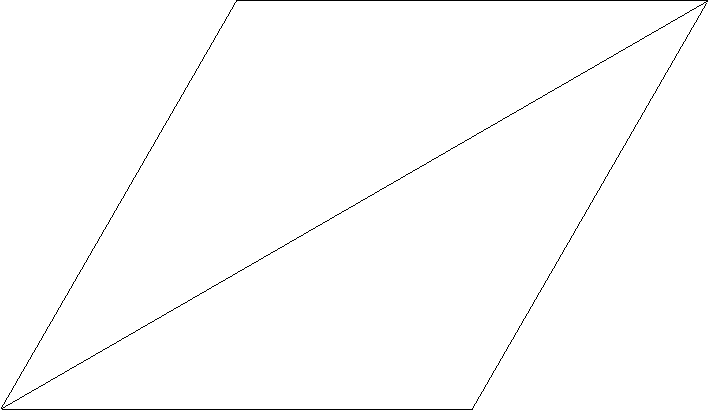
\includegraphics[width=5cm]{workingExample1}
    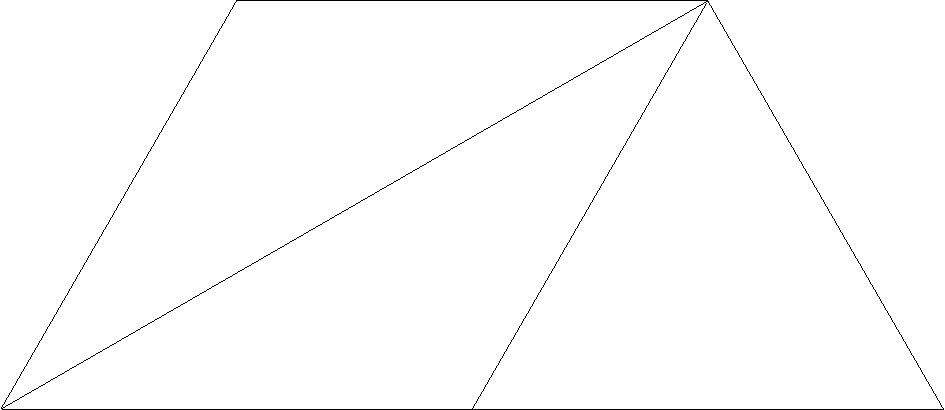
\includegraphics[width=5cm]{workingExample2}
    
\includegraphics[width=5cm]{ideal2}
    \caption{Cones of the progressive computation for the \grob fan of the ideal
      $\{yz + x, xy + z, x^2 -z^2\}$}
  \end{figure}

  Using the \emph{gfanInterface} \cite{gfan} from Macaulay2 \cite{M2} we observe the render produced
  intersect the cone with the hyper-plane $x + y + z = 1$ in order to produce a 2D plot. From this
  fact we know the set of cones cover the positive orthant of $\real^3$ when the render forms a triangle.
  Hence, we can choose a vector ($w = (1, 0, 0)$) from the bottom right side. From the latter
  we obtain the marked \grob basis (the correspondent set of cones is in Figure 2 (Center)) $\{(y^2*z) -z, (x) + y*z\}$.
  Now we try to extend the cones with the vector $w = (0, 0, 1)$ and we obtain the marked \grob
  basis $\{(x*y^2) -x, (z) + x*y\}$. The final set of cones is shown in Figure 2 (Right). Since
  the latter intersects with the triangle mention before we are sure we have computed all the
  marked \grob bases for the ideal $\{yz + x, xy + z, x^2 -z^2\}$.
\end{example}


%%% Local Variables:
%%% mode: latex
%%% TeX-master: "main"
%%% End:

\begin{example}
  Let us consider the polynomial ring $\mathbb{Q}[x, y, z]$ and
  the ideal $\{x*y - x, x^2 + x*z, y^2*z + x\}$. For this example we will
  use our implementation of the Mora and Robbiano algorithm.

  \begin{itemize}
  \item First we compute all the possible monomial orders. Enumerating all the possibilities
    these are the potential candidates:

    \begin{itemize}
    \item $\{(x*y) - x, (x^2) + x*z, (y^2*z) + x\}$
    \item $\{(x*y) - x, (x^2) + x*z, y^2*z + (x)\}$
    \item $\{(x*y) - x, x^2 + (x*z), (y^2*z) + x\}$
    \item $\{(x*y) - x, x^2 + (x*z), y^2*z + (x)\}$
    \item $\{x*y - (x), (x^2) + x*z, (y^2*z) + x\}$
    \item $\{x*y - (x), (x^2) + x*z, y^2*z + (x)\}$
    \item $\{x*y - (x), x^2 + (x*z), (y^2*z) + x\}$
    \item $\{x*y - (x), x^2 + (x*z), y^2*z + (x)\}$
    \end{itemize}

    However, not all the previous candidates will define monomial orders. Using a linear
    programming solver we obtain the following set of polynomials that define
    a monomial order:
    
    \begin{itemize}
    \item $\{(x*y) - x, (x^2) + x*z, (y^2*z) + x\}$
    \item $\{(x*y) - x, (x^2) + x*z, y^2*z + (x)\}$
    \item $\{(x*y) - x, x^2 + (x*z), (y^2*z) + x\}$
    \end{itemize}

  \item Now we extend each set of polynomials to marked \grob bases.
    We obtain:

    \begin{itemize}
    \item $\{(x*y) - x, x^2 + (x*z), (y^2*z) + x\}$
    \item $\{(x*y) - x, (x^2) + x*z, y^2*z + x, (-y^3*z) + y^2*z\}$
    \item $\{(x*y) - x, (x^2) + x*z, (y^2*z) + x\}$
    \end{itemize}

  \item Finally, we obtain the reduced marked \grob basis, this step help
    to eliminate marked \grob bases than define the same monomial order.
    In this case, we kept the same number of reduced marked \grob basis
    but we eliminated redundant polynomials:

    \begin{itemize}
    \item $\{(x^2) + x*z, (x*y) - x, (y^2*z) + x\}$ 
    \item $\{(-y^3*z) + y^2*z, y^2*z + (x)\}$  
    \item $\{x^2 + (x*z), (x*y) - x, (y^2*z) + x\}$
    \end{itemize}
  \end{itemize}
  
  \begin{figure}[h]
    \centering
    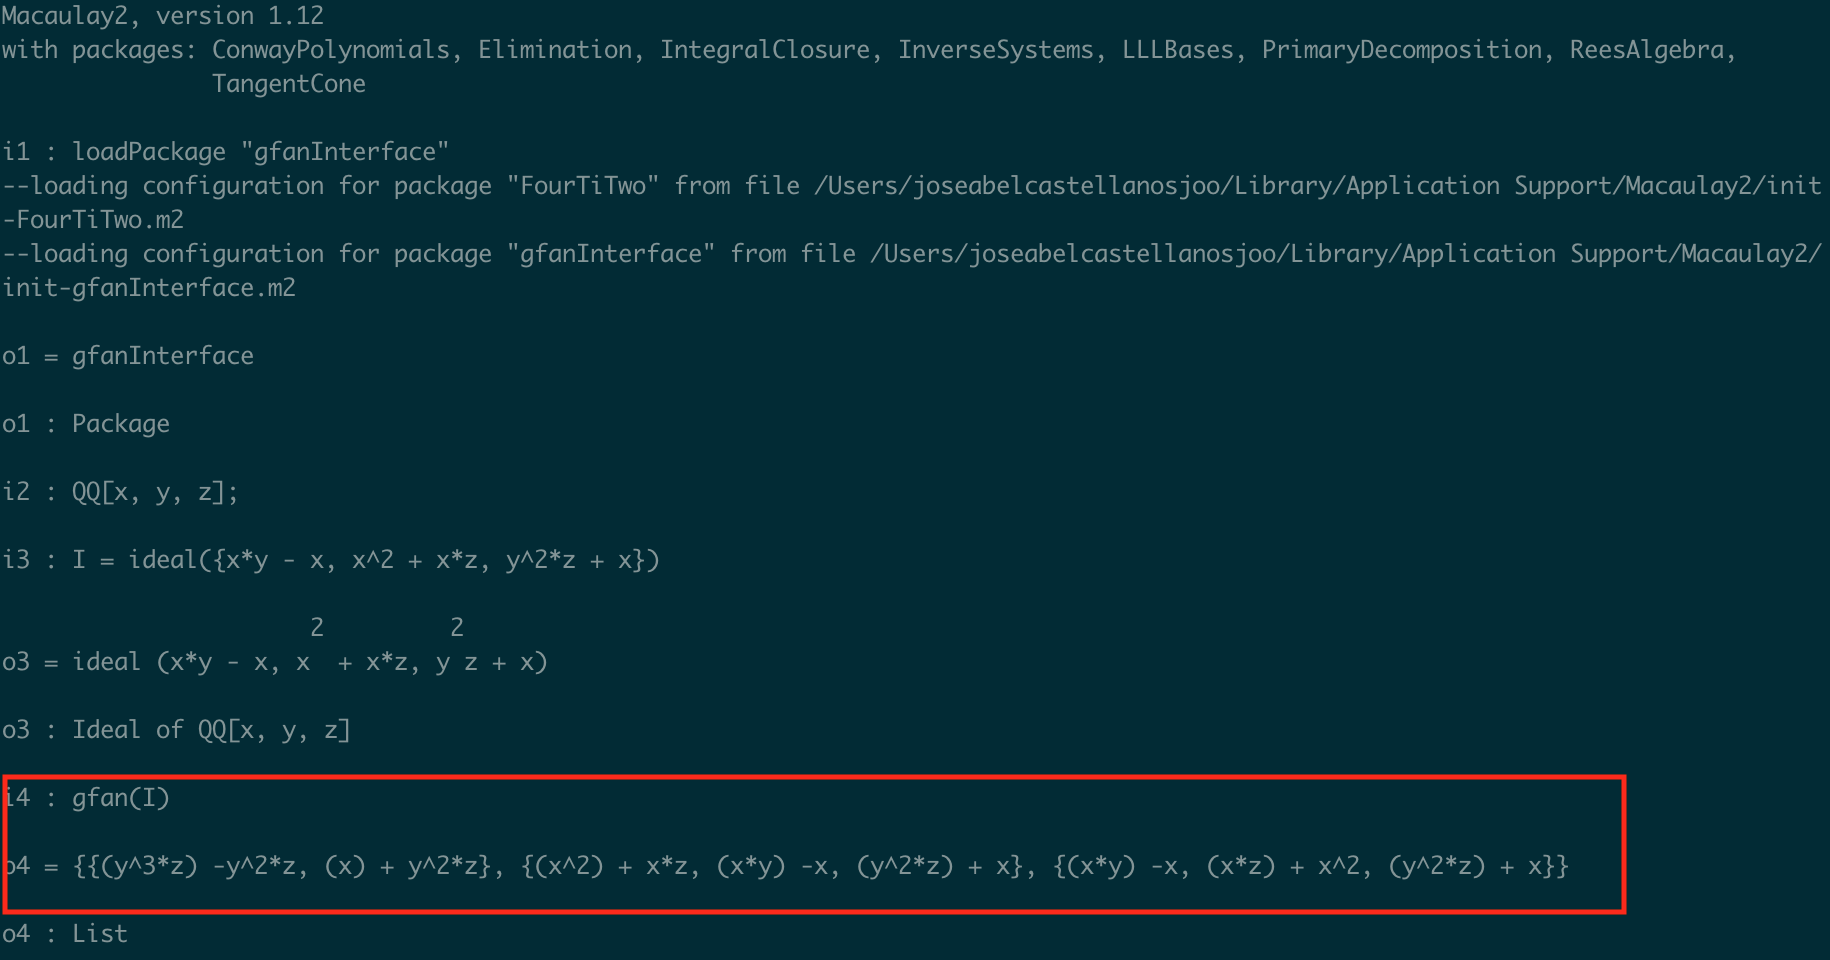
\includegraphics[width=9cm]{gfanIdeal3}
    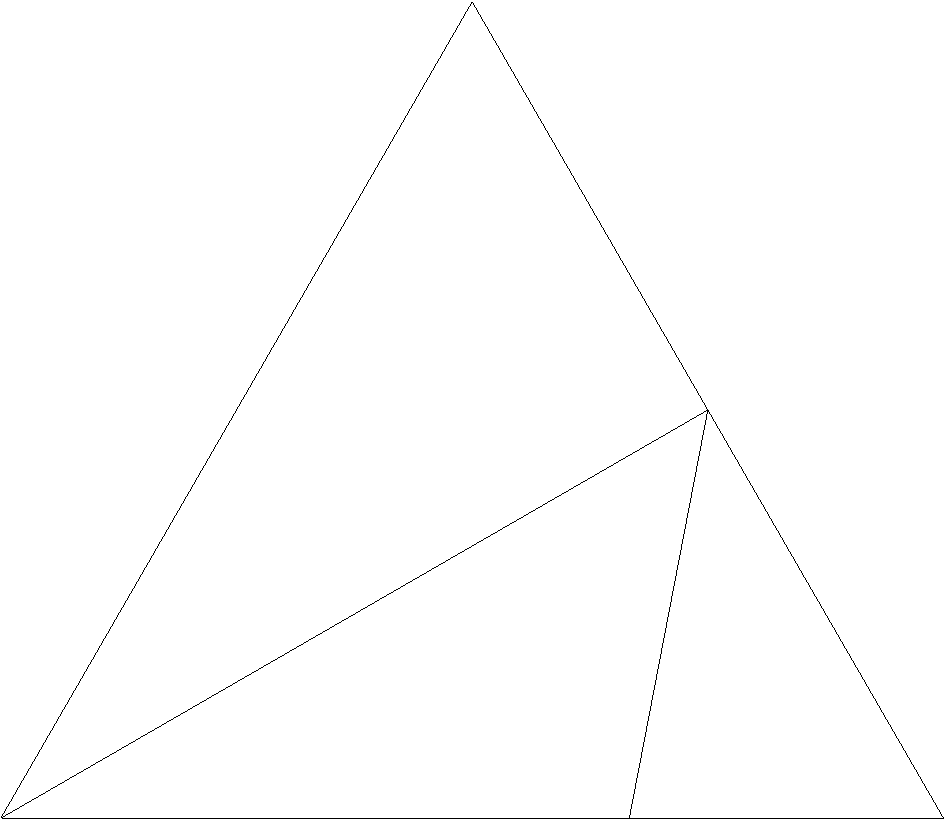
\includegraphics[width=6cm]{ideal3}
    \caption{(Left) Using gfan to compute the \grob fan of the ideal
      $\{x*y - x, x^2 + x*z, y^2*z + x\}$; (Right) Visualization of the \grob
    fan of the ideal $\{x*y - x, x^2 + x*z, y^2*z + x\}$}
  \end{figure}
\end{example}

%%% Local Variables:
%%% mode: latex
%%% TeX-master: "main"
%%% End:

\begin{example}
  Let us consider the polynomial ring $\mathbb{Q}[x, y, z]$ and
  the ideal $\{x^2  - y, y^2  - x*z - y*z\}$. For this example we will
  use our implementation of the Mora and Robbiano algorithm. We will
  repeat the same steps as in the previous example highlighting the output
  produced at each step:

  \begin{itemize}
  \item Valid monomial orders:

    \begin{itemize}
      \item $\{(x^2) - y, (y^2) - x*z - y*z\}$ 
      \item $\{(x^2) - y, y^2 - (x*z) - y*z\}$ 
      \item $\{(x^2) - y, y^2 - x*z - (y*z)\}$ 
      \item $\{x^2 - (y), (y^2) - x*z - y*z\}$ 
      \item $\{x^2 - (y), y^2 - x*z - (y*z)\}$ 
    \end{itemize}

  \item Marked \grob basis:

    \begin{itemize}
      \item $\{x^2 - (y), y^2 - x*z - (y*z), x^4 - (x^2*z) - x*z\}$
      \item $\{x^2 - (y), (y^2) - x*z - y*z, x^4 - (x^2*z) - x*z\}$
      \item $\{x^2 - (y), (y^2) - x*z - y*z, (x^4) - x^2*z - x*z\}$
      \item $\{(x^2) - y, y^2 - x*z - (y*z)\}$
      \item $\{(x^2) - y, y^2 - (x*z) - y*z, -x*y^2 + y^3 - (y^2*z) + y*z\}$
      \item $\{(x^2) - y, y^2 - (x*z) - y*z, (-x*y^2) + y^3 - y^2*z + y*z, -y^4 + 2*y^3*z - (y^2*z^2) + y*z^2\}$
      \item $\{(x^2) - y, y^2 - (x*z) - y*z, (-x*y^2) + y^3 - y^2*z + y*z, (-y^4) + 2*y^3*z - y^2*z^2 + y*z^2\}$
      \item $\{(x^2) - y, (y^2) - x*z - y*z\}$
    \end{itemize}

  \item Reduced marked \grob basis:

    \begin{itemize}
      \item $\{(y^2) - x*z - y*z, (x^2) - y\}$
      \item $\{y^2 - (x*z) - y*z, (-y^4) + 2*y^3*z - y^2*z^2 + y*z^2, (x*y^2) - y^3 + y^2*z - y*z, (x^2) - y\}$
      \item $\{y^2 - (x*z) - y*z, -y^4 + 2*y^3*z - (y^2*z^2) + y*z^2, (x*y^2) - y^3 + y^2*z - y*z, (x^2) - y\}$
      \item $\{y^2 - (x*z) - y*z, (x^2) - y, x*y^2 - y^3 + (y^2*z) - y*z\}$
      \item $\{y^2 - x*z - (y*z), (x^2) - y\}$
      \item $\{(x^4) - x^2*z - x*z, -x^2 + (y)\}$
      \item $\{x^4 - (x^2*z) - x*z, -x^2 + (y)\}$
    \end{itemize}
  \end{itemize}
  
  \begin{figure}[h]
    \centering
    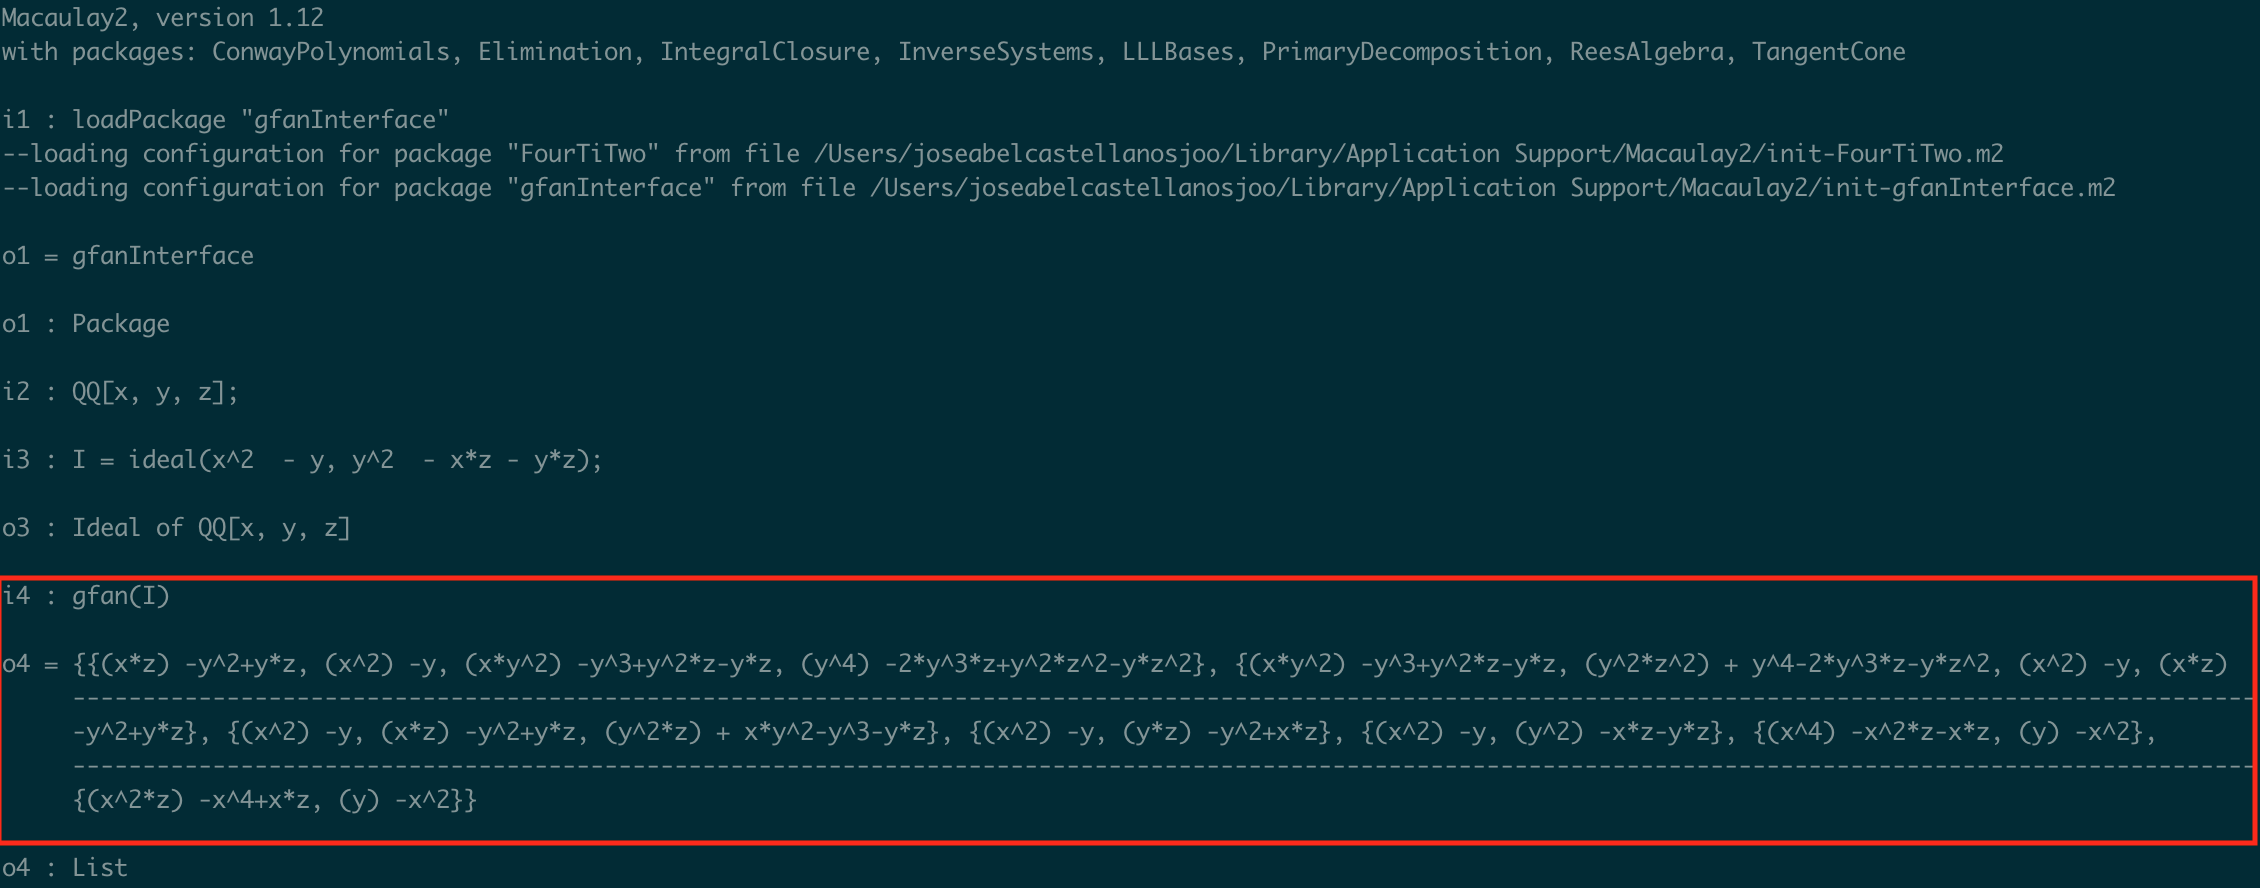
\includegraphics[width=9cm]{gfanIdeal1}
    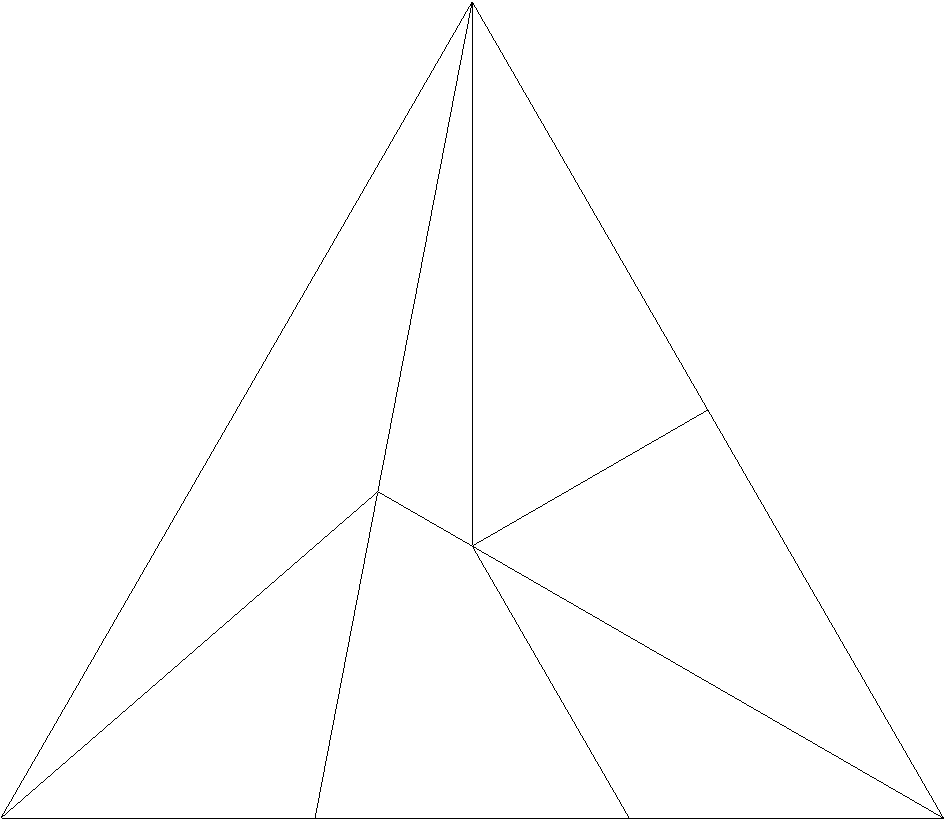
\includegraphics[width=6cm]{ideal1}
    \caption{(Left) Using gfan to compute the \grob fan of the ideal
      $\{x^2  - y, y^2  - x*z - y*z\}$; (Right) Visualization of the \grob
    fan of the ideal $\{x^2  - y, y^2  - x*z - y*z\}$}
  \end{figure}
\end{example}


%%% Local Variables:
%%% mode: latex
%%% TeX-master: "main"
%%% End:


%%% Local Variables: 
%%% mode: latex
%%% TeX-master: "main"
%%% End: 
\section{Conclusion}

Blah Blahhhhh

\bibliographystyle{unsrt}
\bibliography{reference}

\end{document}